\subsection{تخمین پارامتر کانال رول}
برای اصلاح پارامترها رول چندین آزمایش انجام شد و با استفاده از خروجی آزمایش و جعبه‌ابزاز
\lr{Parameter Estimator}
پارامترها اصلاح شدند.
برای آزمایش رول هر یک از موتورها با دور مختلف شروع به حرکت کردند و خروجی سنسور داده برداری شد. سپس، مدل و پارامترهای داده برداری شده به جعبه‌ابزار
\lr{Parameter Estimator}
داده شد. نتایج آزمایش‌های کانال رول بعد از اصلاح پارامترها در شکل‌های
()
آورده شده است.

\begin{figure}[H]
	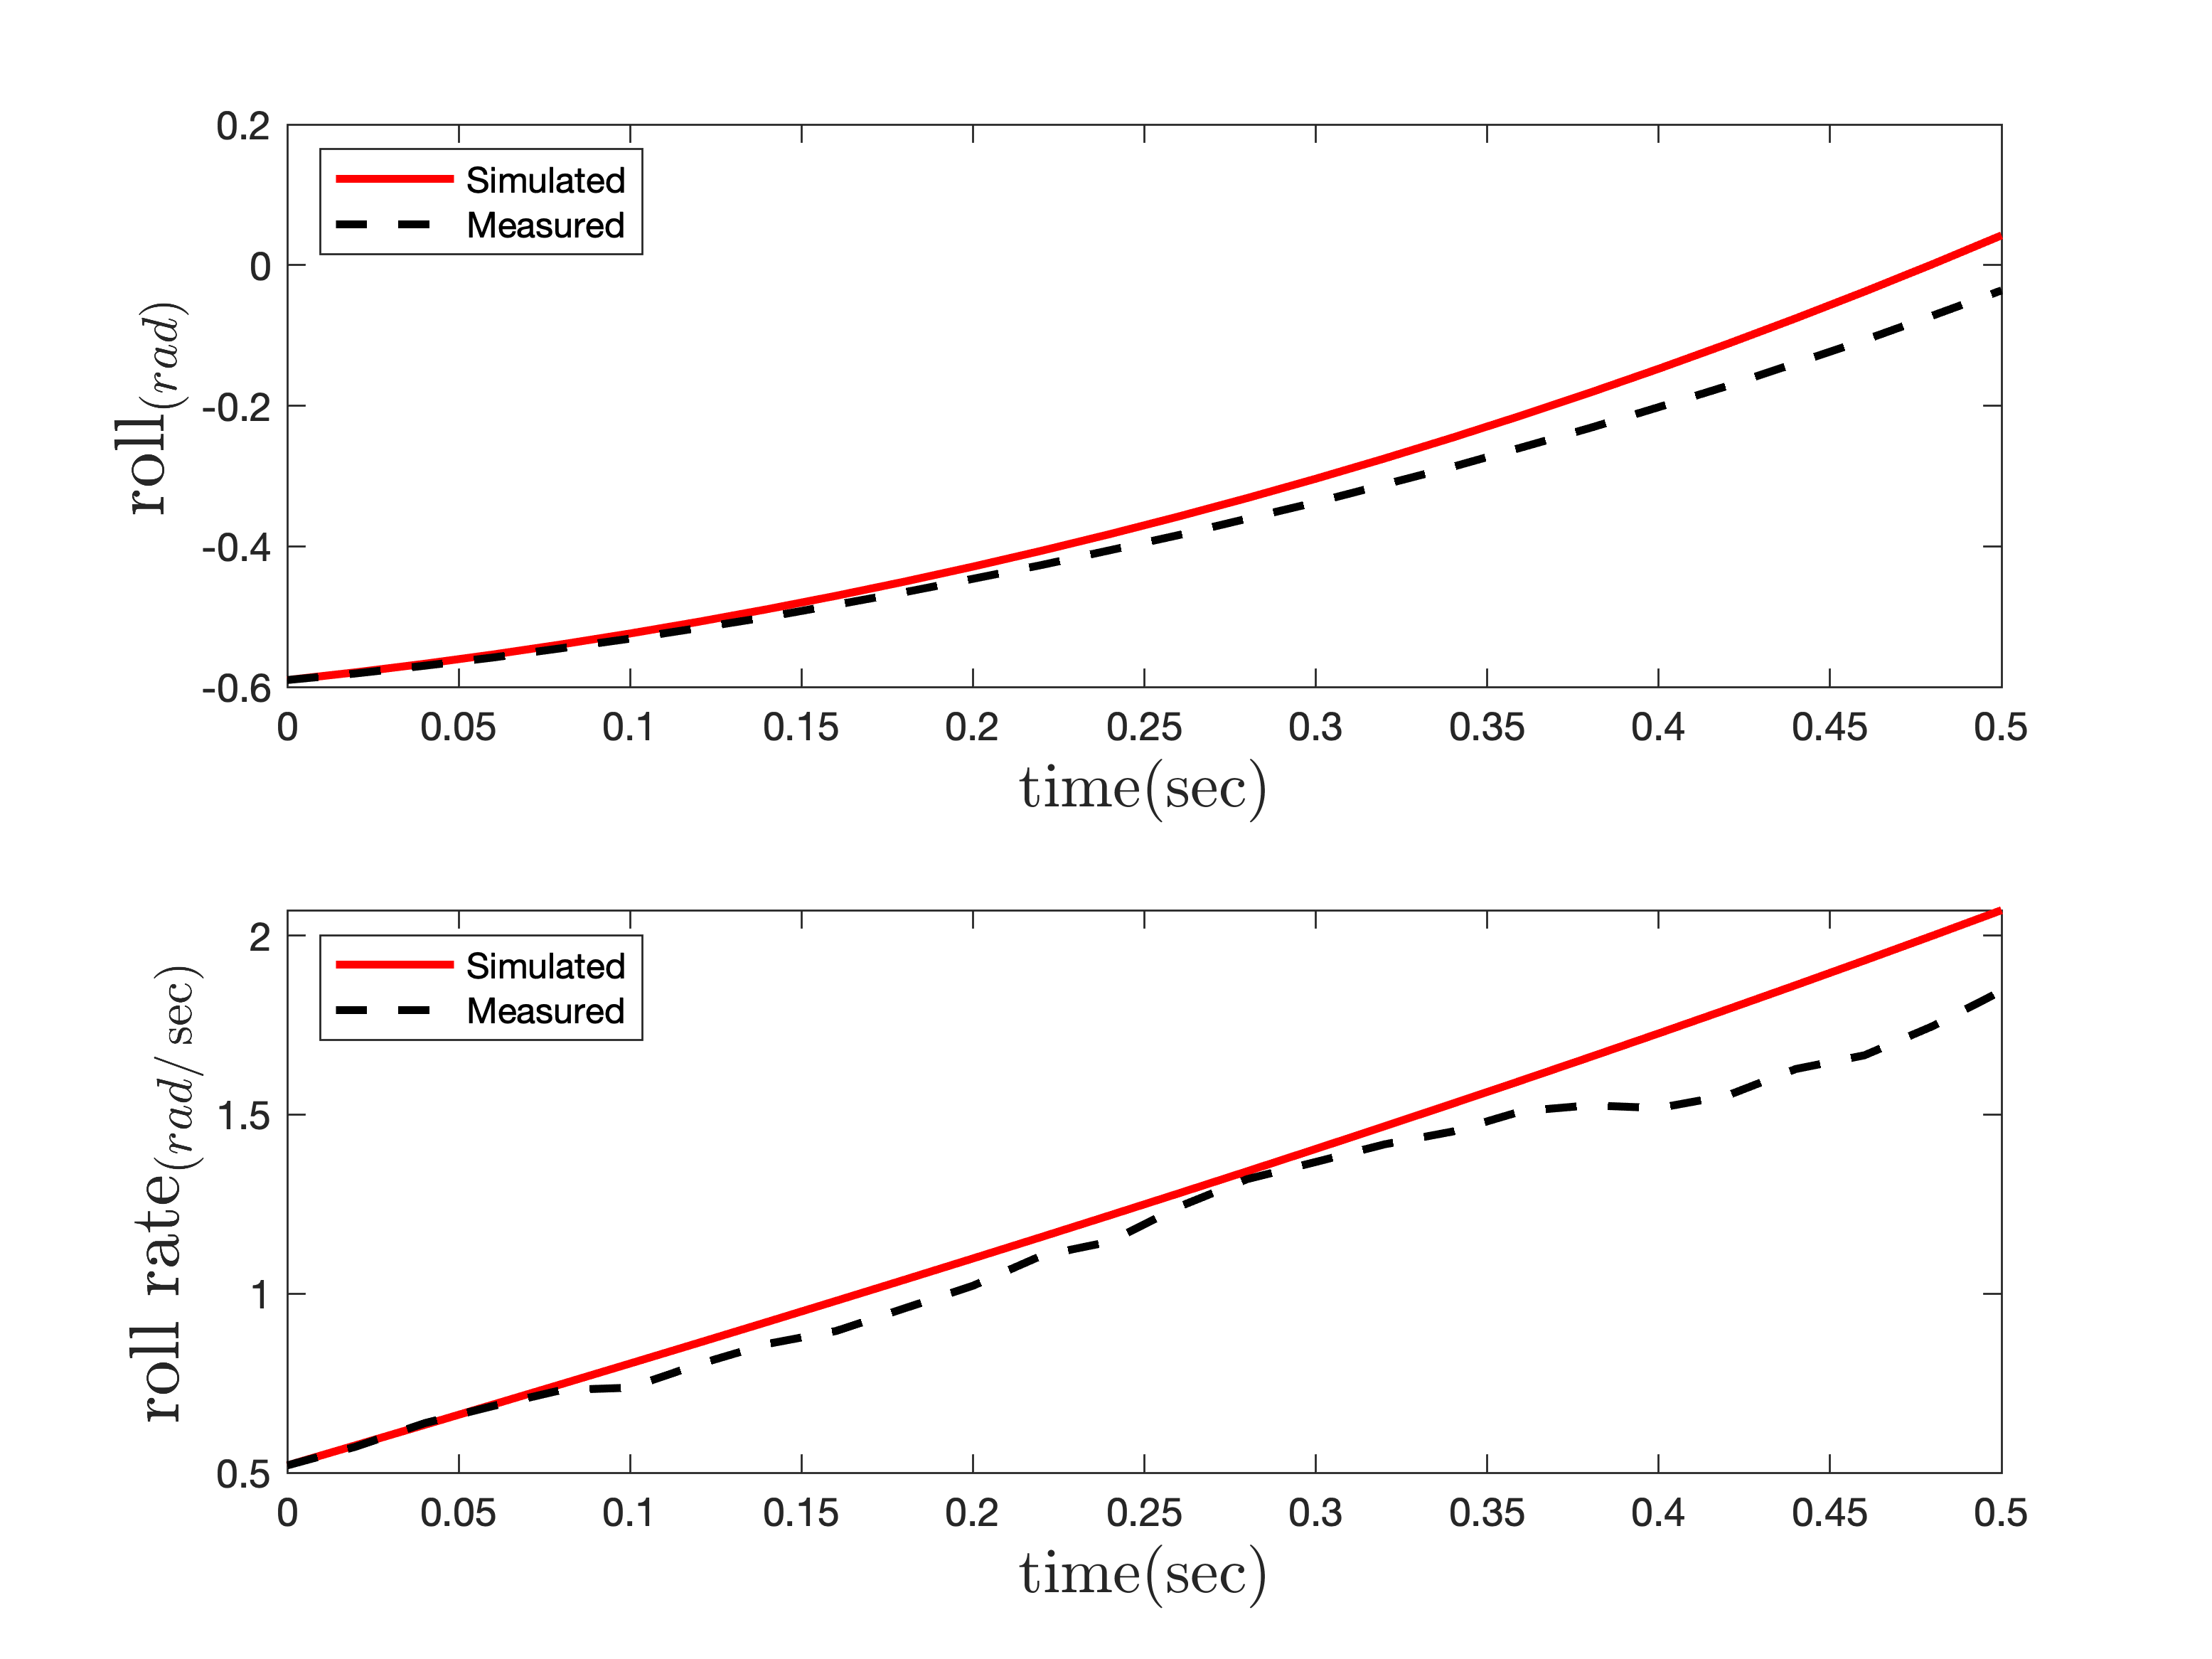
\includegraphics[width=12cm]{../../Figures/RCP/roll_parameter_estimation/RCP_roll_S1.png}
	\centering
	\caption{مقايسه خروجيهای آزمايش اول و خروجي مدلسازی پس از تخمین پارامترها}
	\label{roll_ps1}
\end{figure}
\begin{figure}[H]
	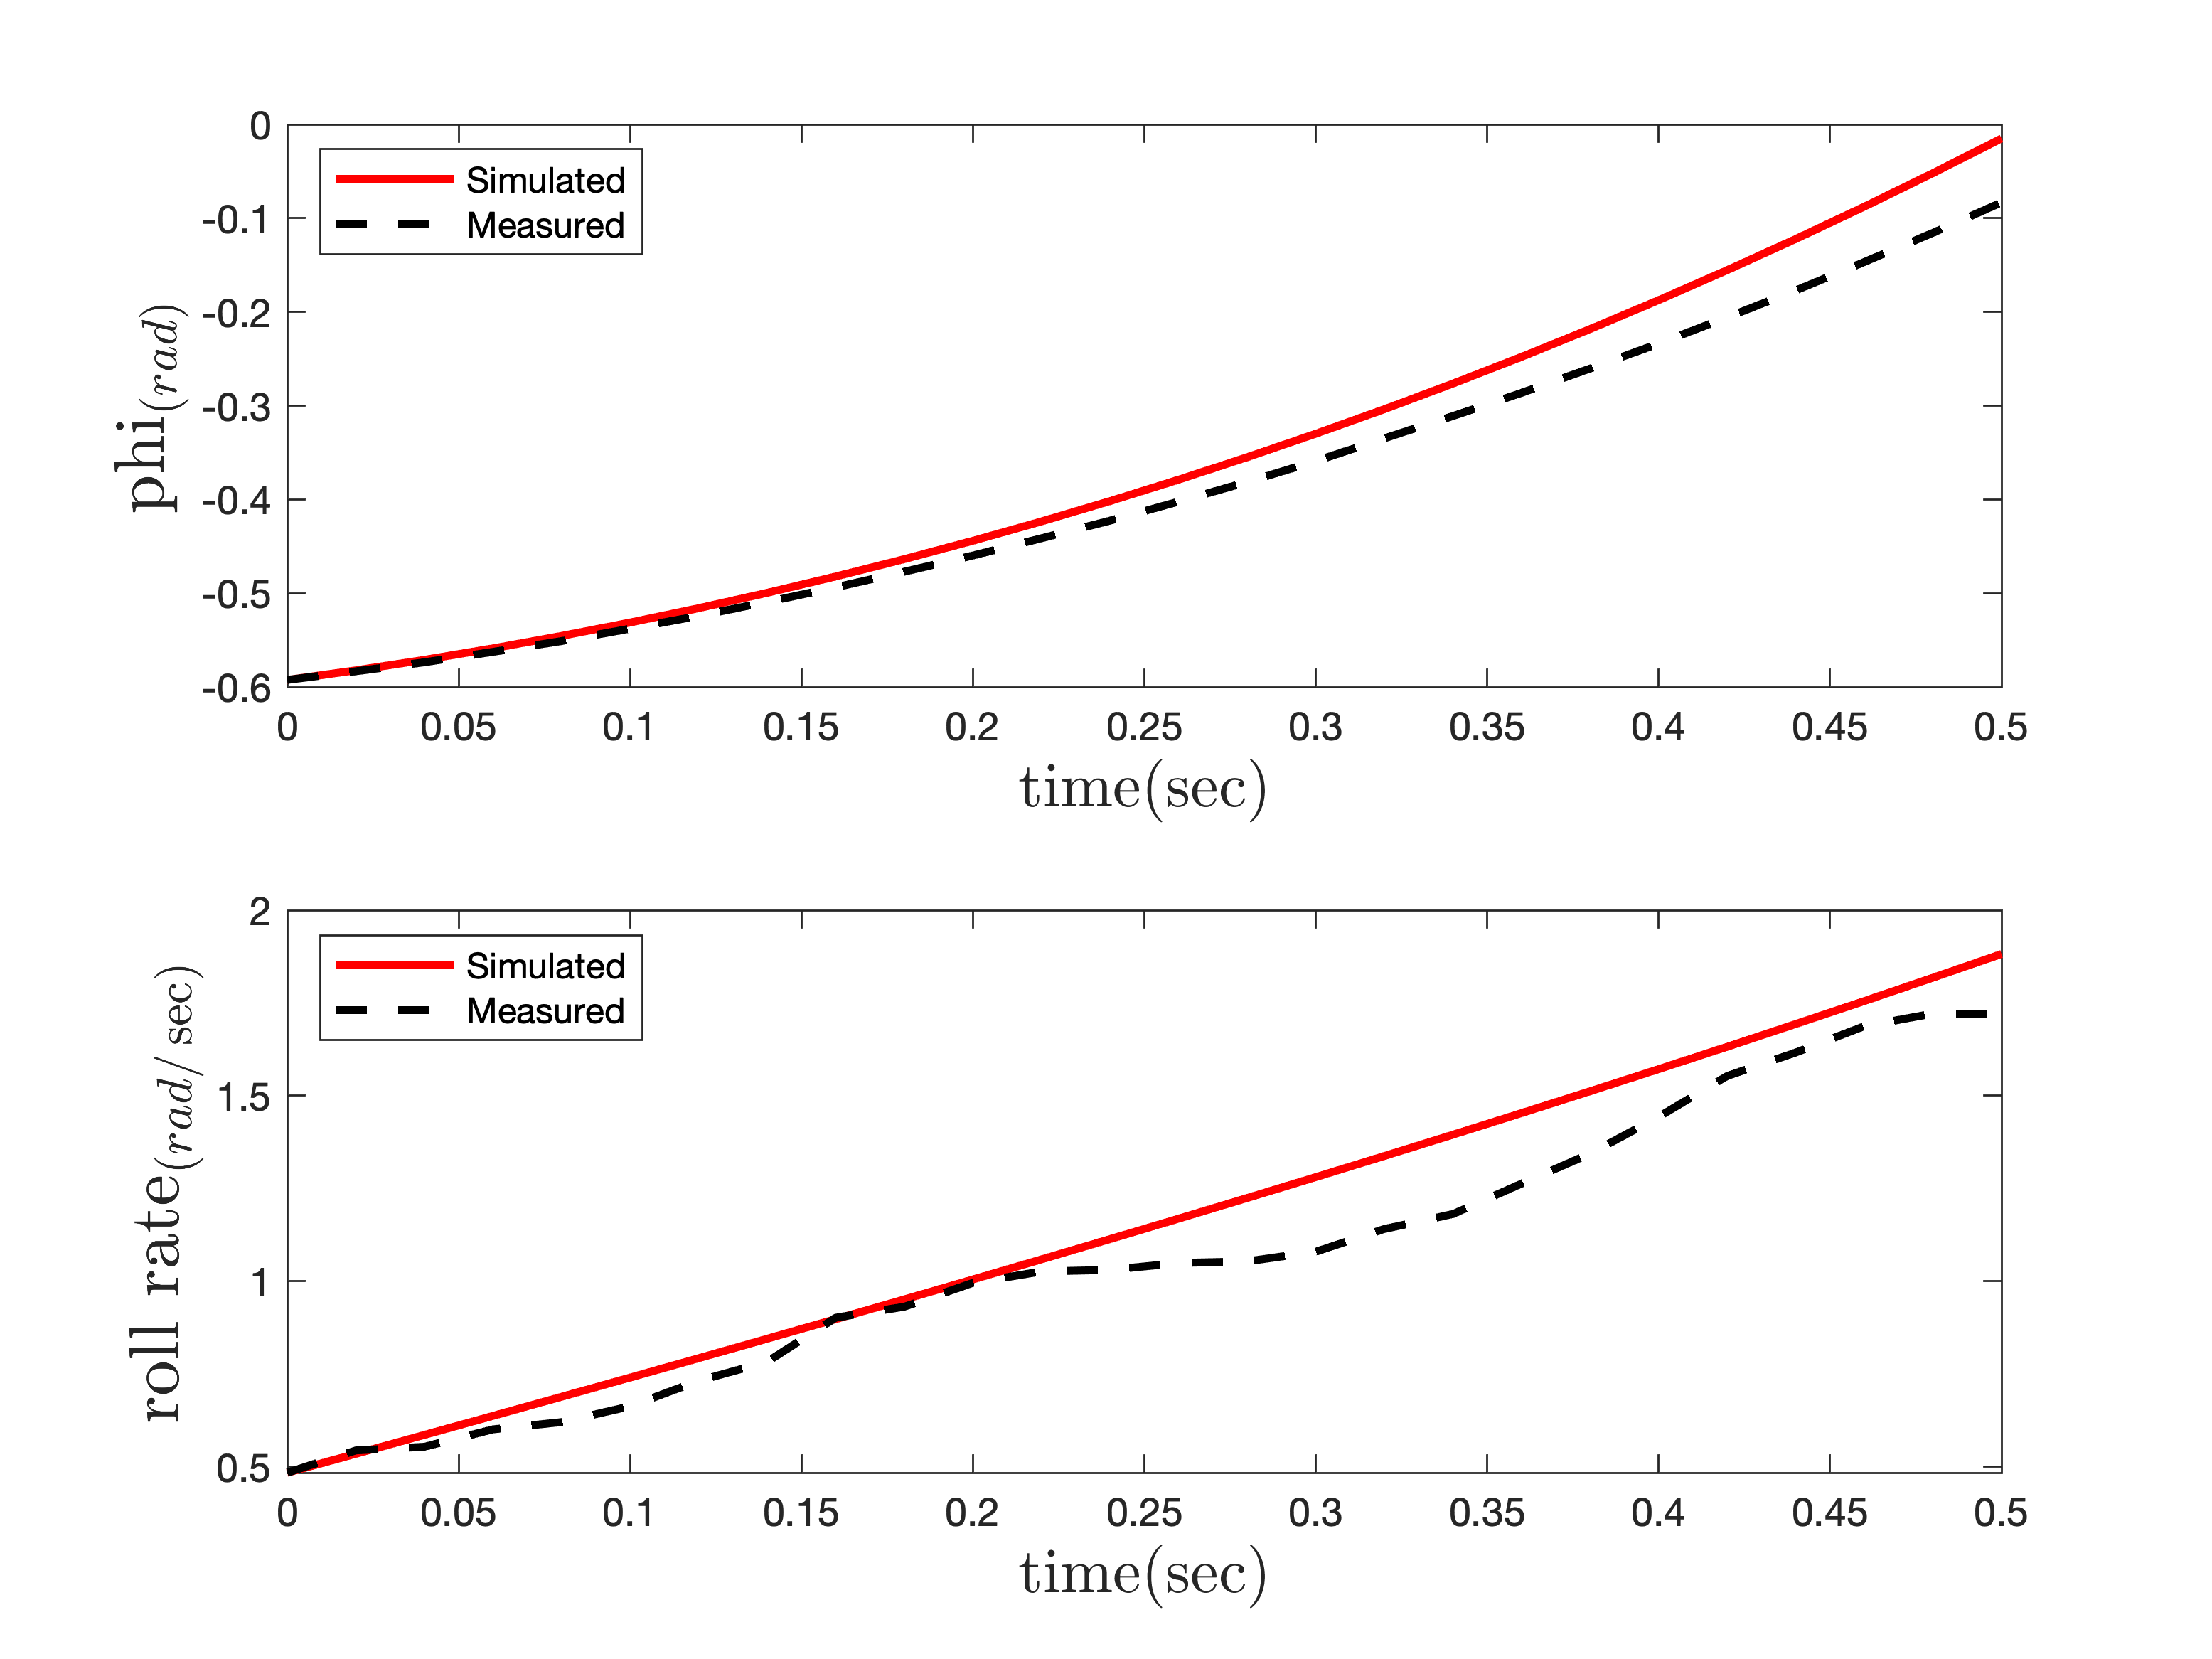
\includegraphics[width=12cm]{../../Figures/RCP/roll_parameter_estimation/RCP_roll_S2.png}
	\centering
	\caption{مقايسه خروجيهای آزمايش دوم و خروجي مدلسازی پس از تخمین پارامترها}
	\label{roll_ps2}
\end{figure}
\begin{figure}[H]
	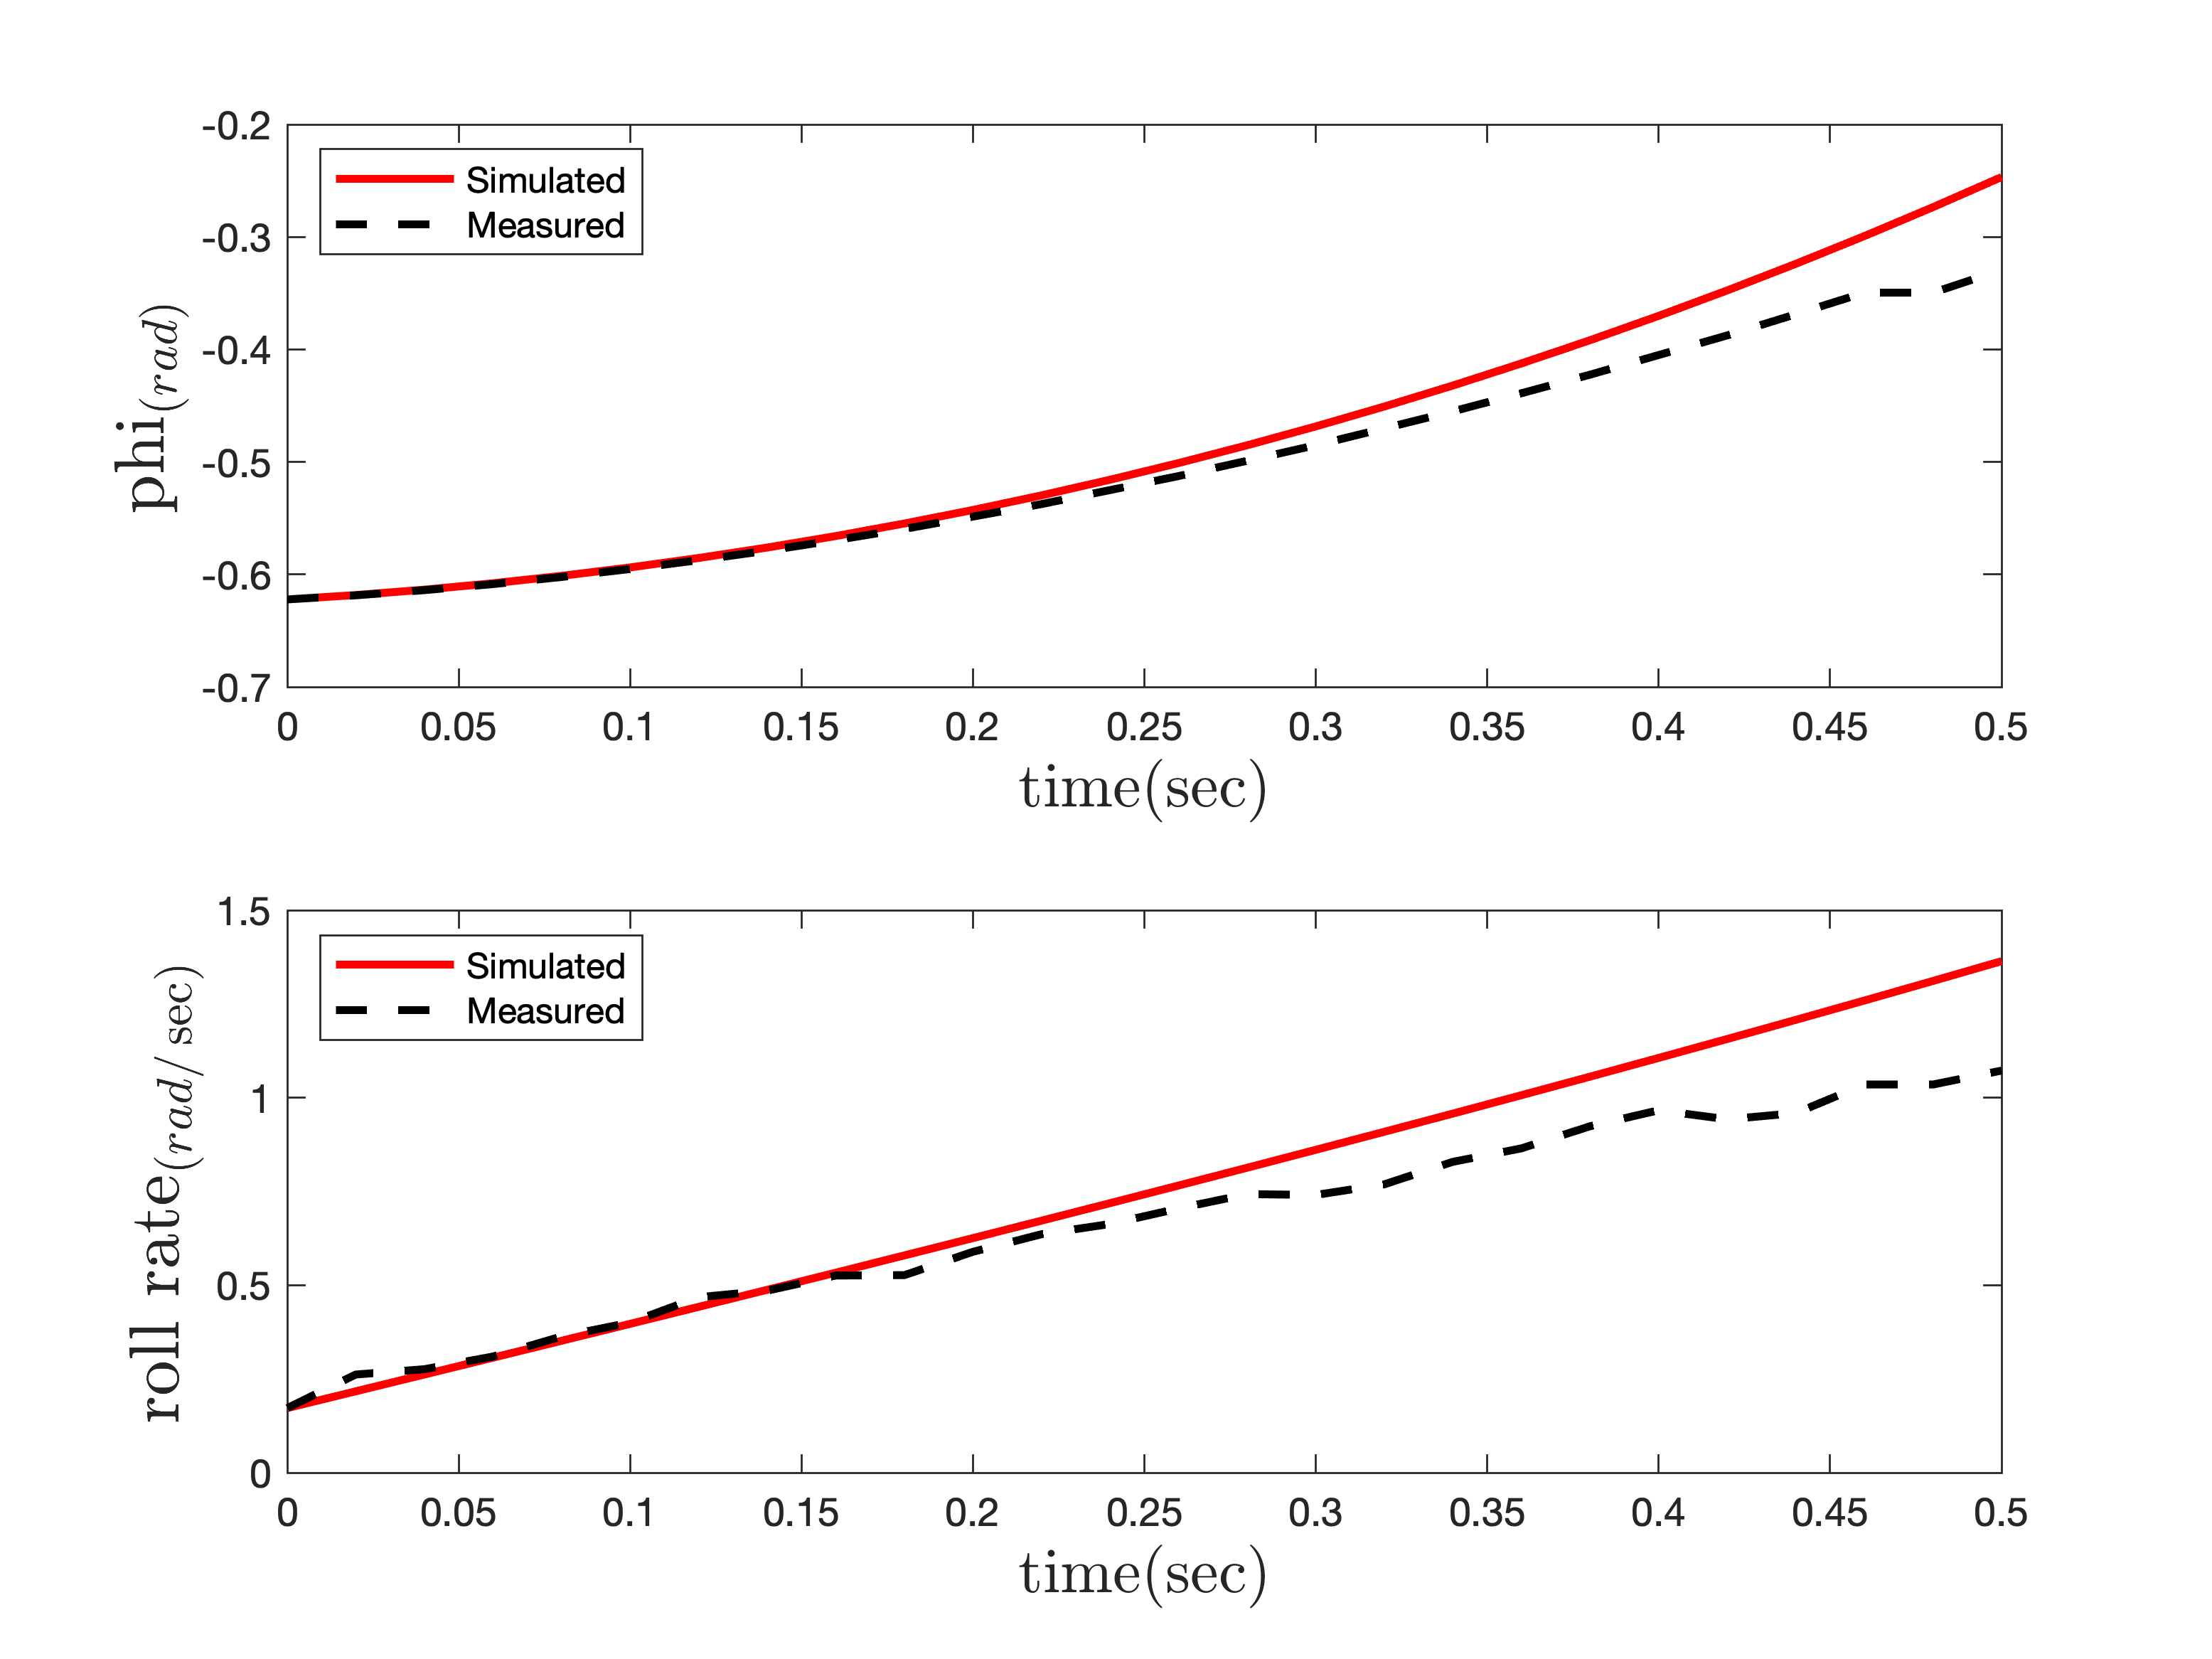
\includegraphics[width=12cm]{../../Figures/RCP/roll_parameter_estimation/RCP_roll_S3.png}
	\centering
	\caption{مقايسه خروجيهای آزمايش سوم و خروجي مدلسازی پس از تخمین پارامترها}
	\label{roll_ps3}
\end{figure}
\begin{figure}[H]
	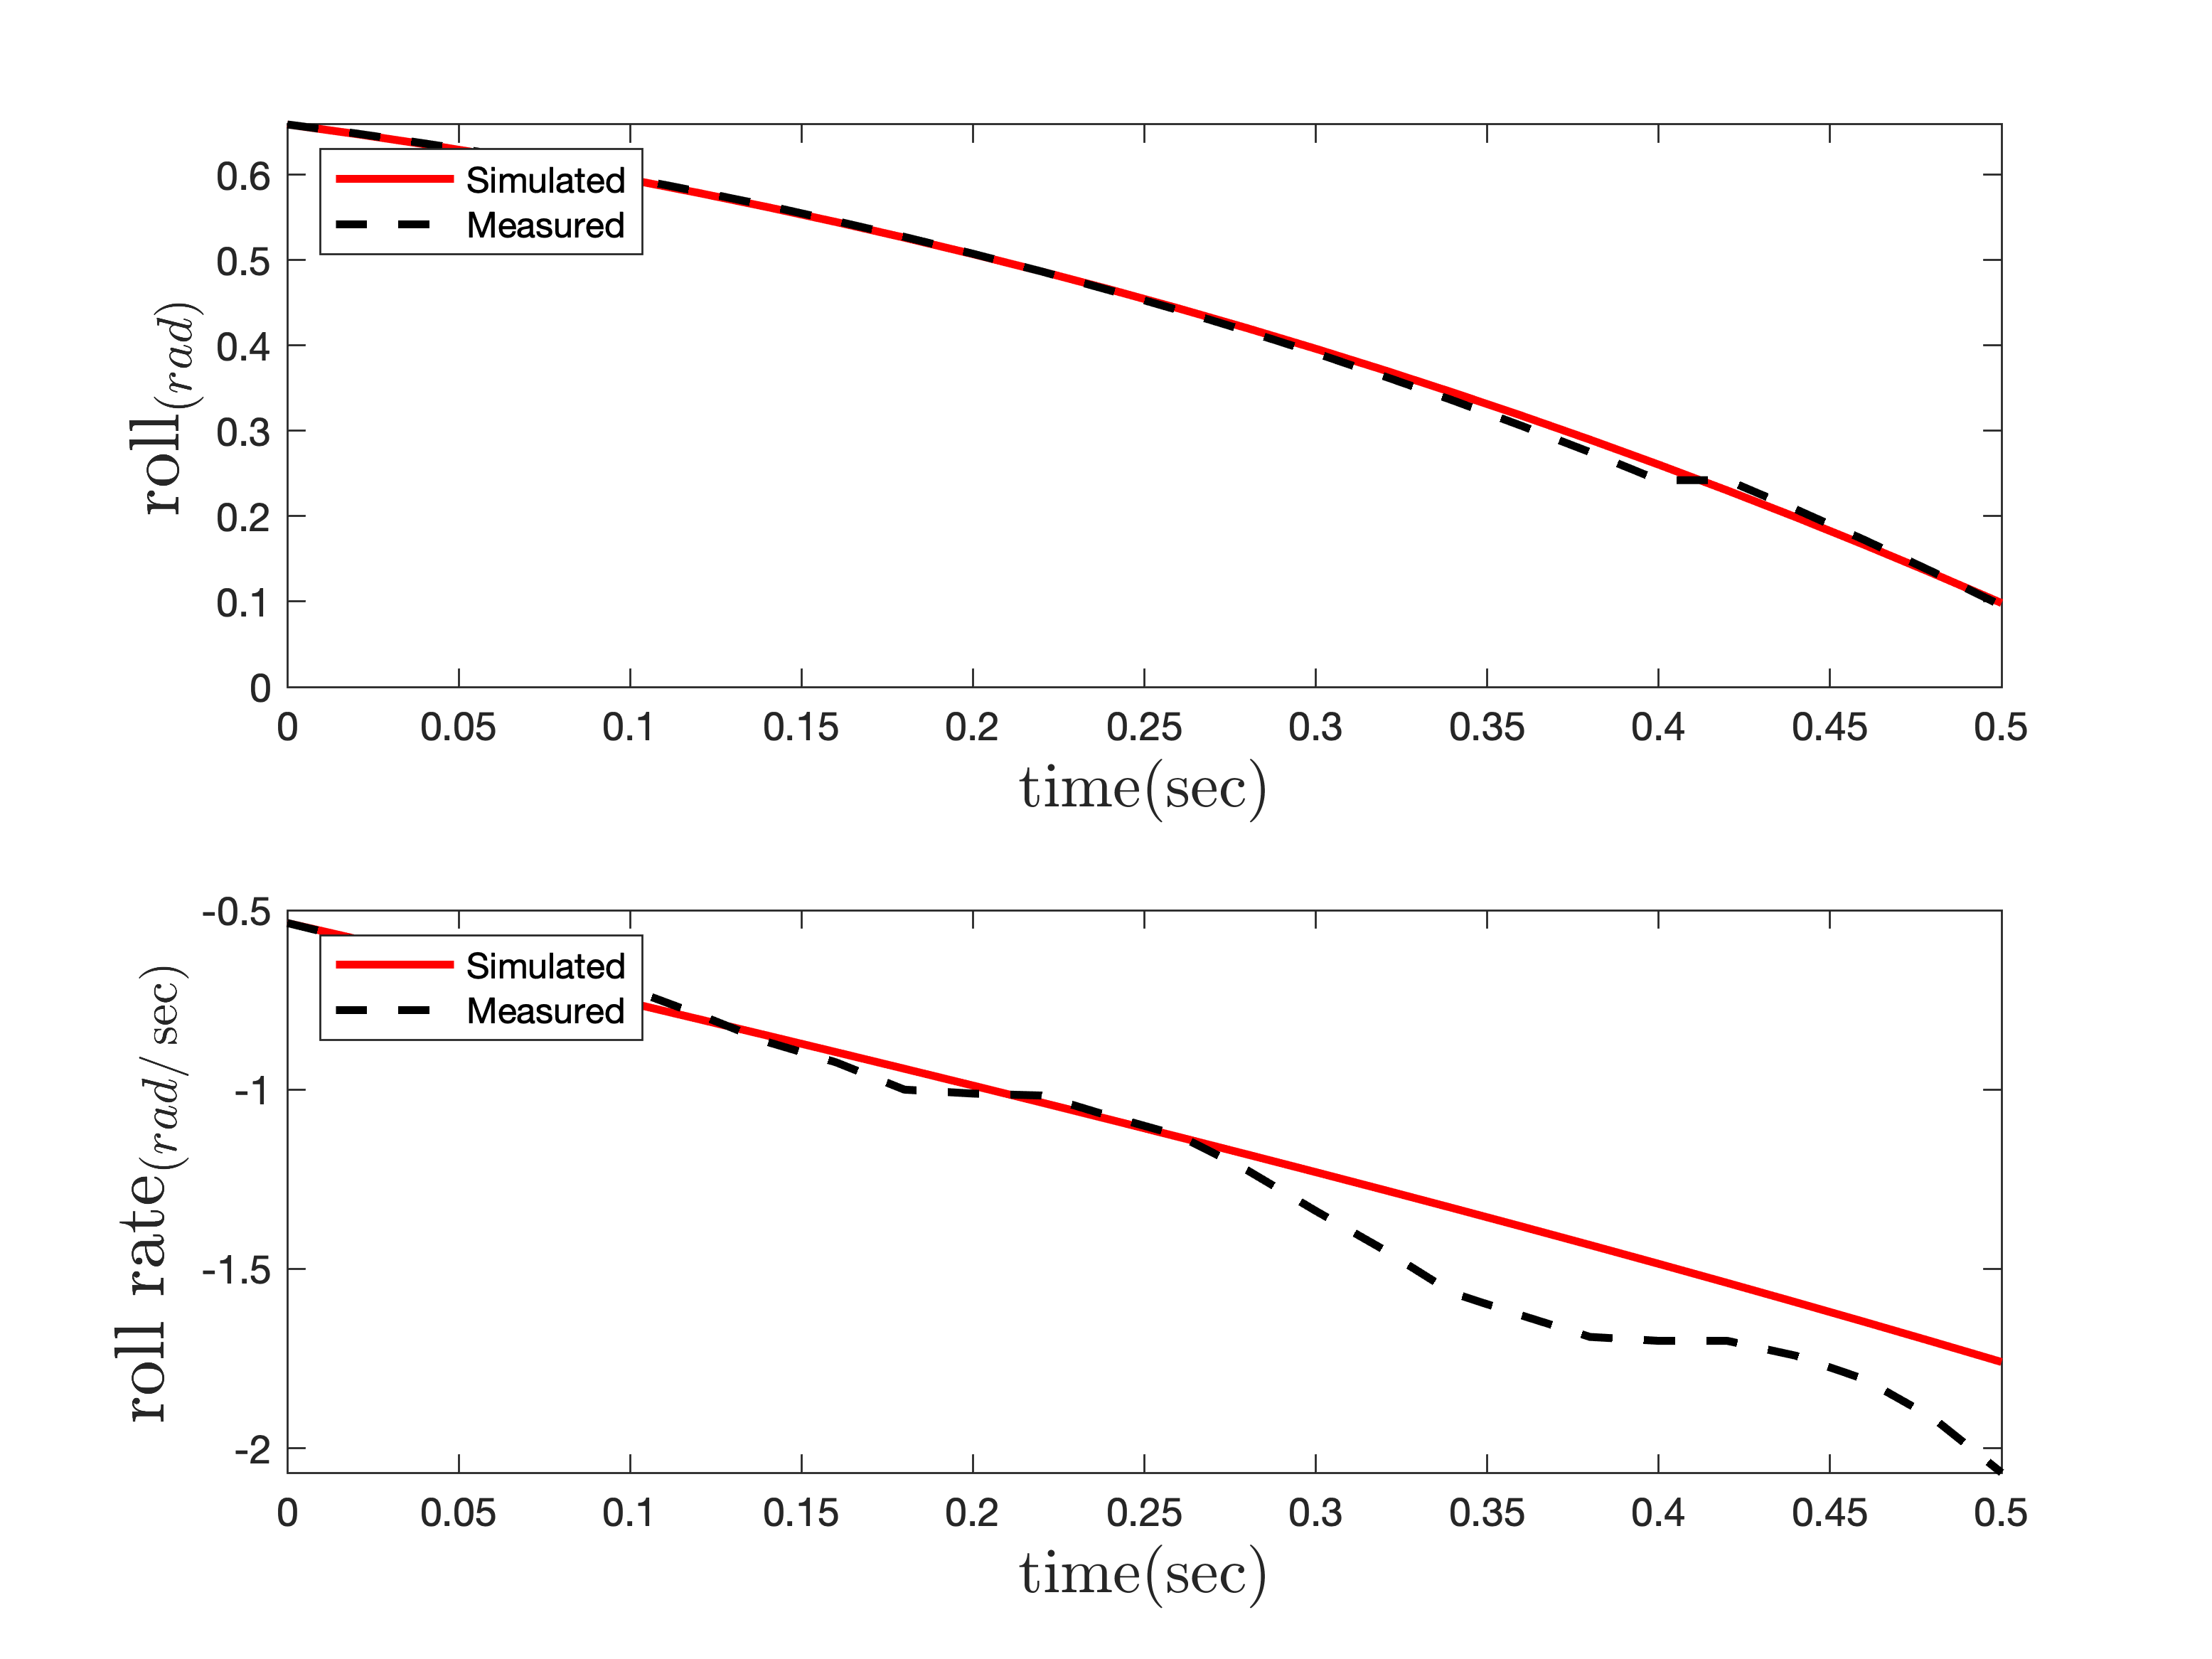
\includegraphics[width=12cm]{../../Figures/RCP/roll_parameter_estimation/RCP_roll_S4.png}
	\centering
	\caption{مقايسه خروجيهای آزمايش چهارم و خروجي مدلسازی پس از تخمین پارامترها}
	\label{roll_ps4}
\end{figure}
\begin{figure}[H]
	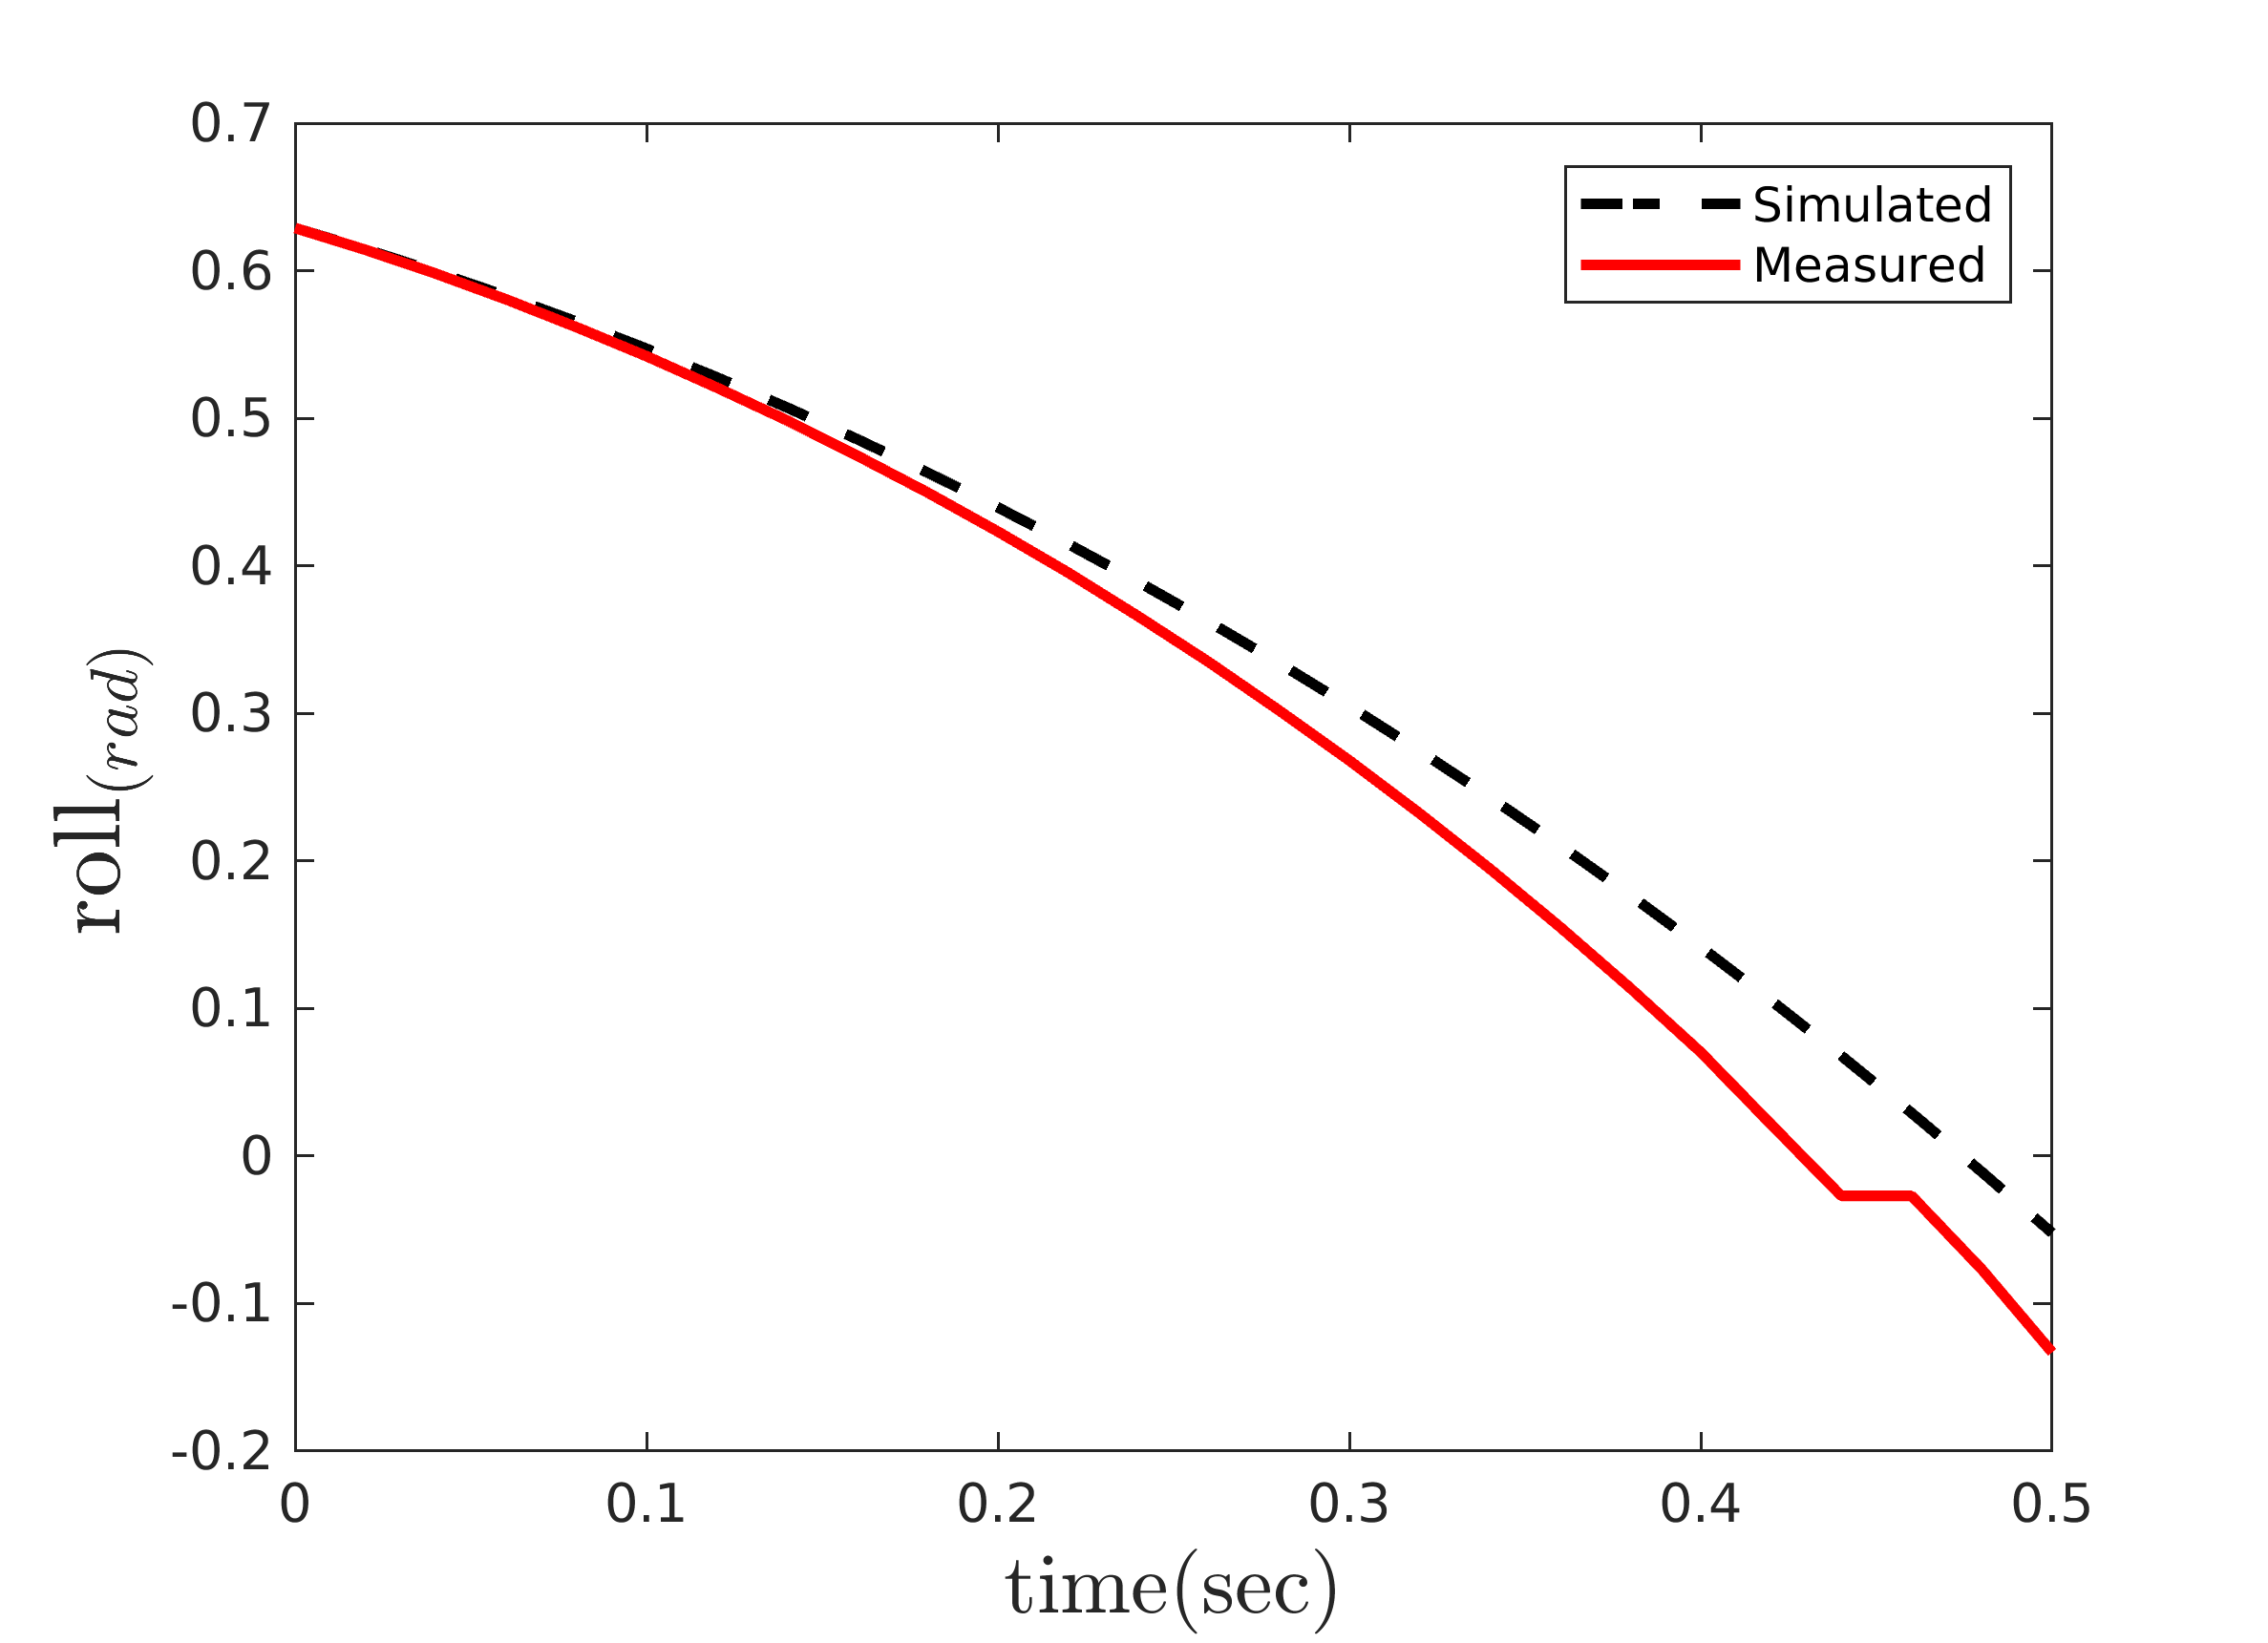
\includegraphics[width=12cm]{../../Figures/RCP/roll_parameter_estimation/RCP_roll_S5.png}
	\centering
	\caption{مقايسه خروجيهای آزمايش پنجم و خروجي مدلسازی پس از تخمین پارامترها}
	\label{roll_ps5}
\end{figure}